% --- Template for thesis / report with tktltiki2 class ---

\documentclass[finnish]{../tktltiki2}

% tktltiki2 automatically loads babel, so you can simply
% give the language parameter (e.g. finnish, swedish, english, british) as
% a parameter for the class: \documentclass[finnish]{tktltiki2}.
% The information on title and abstract is generated automatically depending on
% the language, see below if you need to change any of these manually.
% 
% Class options:
% - grading                 -- Print labels for grading information on the front page.
% - disablelastpagecounter  -- Disables the automatic generation of page number information
%                              in the abstract. See also \numberofpagesinformation{} command below.
%
% The class also respects the following options of article class:
%   10pt, 11pt, 12pt, final, draft, oneside, twoside,
%   openright, openany, onecolumn, twocolumn, leqno, fleqn
%
% The default font size is 11pt. The paper size used is A4, other sizes are not supported.
%
% rubber: module pdftex

% --- General packages ---

\usepackage[utf8]{inputenc}
\usepackage{lmodern}
\usepackage{microtype}
\usepackage{amsfonts,amsmath,amssymb,amsthm,booktabs,color,enumitem,graphicx}
\usepackage[pdftex,hidelinks]{hyperref}

% Automatically set the PDF metadata fields
\makeatletter
\AtBeginDocument{\hypersetup{pdftitle = {\@title}, pdfauthor = {\@author}}}
\makeatother

% --- Language-related settings ---
%
% these should be modified according to your language

% babelbib for non-english bibliography using bibtex
\usepackage[fixlanguage]{babelbib}
\selectbiblanguage{finnish}

% add bibliography to the table of contents
\usepackage[nottoc]{tocbibind}
% tocbibind renames the bibliography, use the following to change it back
\settocbibname{Lähteet}

% --- Theorem environment definitions ---

\newtheorem{lau}{Lause}
\newtheorem{lem}[lau]{Lemma}
\newtheorem{kor}[lau]{Korollaari}

\theoremstyle{definition}
\newtheorem{maar}[lau]{Määritelmä}
\newtheorem{ong}{Ongelma}
\newtheorem{alg}[lau]{Algoritmi}
\newtheorem{esim}[lau]{Esimerkki}

\theoremstyle{remark}
\newtheorem*{huom}{Huomautus}


% --- tktltiki2 options ---
%
% The following commands define the information used to generate title and
% abstract pages. The following entries should be always specified:

\setcounter{secnumdepth}{2}
\setcounter{tocdepth}{2}

\title{Ohjelmistoala ja ryhmätyöskentely}
\author{Kenny Heinonen}
\date{\today}
\level{Aine}
\abstract{Tiivistelmä.}

% The following can be used to specify keywords and classification of the paper:

\keywords{avainsana 1, avainsana 2, avainsana 3}
\classification{} % classification according to ACM Computing Classification System (http://www.acm.org/about/class/)
                  % This is probably mostly relevant for computer scientists

% If the automatic page number counting is not working as desired in your case,
% uncomment the following to manually set the number of pages displayed in the abstract page:
%
% \numberofpagesinformation{16 sivua + 10 sivua liitteissä}
%
% If you are not a computer scientist, you will want to uncomment the following by hand and specify
% your department, faculty and subject by hand:
%
% \faculty{Matemaattis-luonnontieteellinen}
% \department{Tietojenkäsittelytieteen laitos}
% \subject{Tietojenkäsittelytiede}
%
% If you are not from the University of Helsinki, then you will most likely want to set these also:
%
% \university{Helsingin Yliopisto}
% \universitylong{HELSINGIN YLIOPISTO --- HELSINGFORS UNIVERSITET --- UNIVERSITY OF HELSINKI} % displayed on the top of the abstract page
% \city{Helsinki}
%


\begin{document}

% --- Front matter ---

\maketitle        % title page
%\makeabstract     % abstract page

\tableofcontents  % table of contents
\newpage          % clear page after the table of contents


% --- Main matter ---

\section{Johdanto}

Ohjelmistojen kehityksessä ryhmätyöskentely on tärkeää, koska projektien
kasvava kompleksisuus ja laajuus tekee niiden toteuttamisen yksilölle
vaikeaksi~\cite{5593527}.
Ohjelmistoalalla tarvitaan monenlaisia teknisiä taitoja, jotta projekteissa saadaan toteutettua kaikki ohjelmistokehityksen vaiheet 
hyvin. Nämä ohjelmistokehityksen vaiheet voidaan jakaa karkeasti 
vaatimusmäärittelyyn, suunnitteluun, toteutukseen, testaukseen ja 
ylläpitoon~\cite{Capretz:2010:MSS:1726559.1726574}\footnote{Capretz puhuu järjestelmäanalyysista, joka on sidoksissa vaatimusmäärittelyyn. Tässä tekstissä käsitellään järjestelmäanalyysin sijaan vaatimusmäärittelyä.}. Sen lisäksi, että 
eri vaiheet vaativat eri taitoja, myös yksittäinen vaihe kysyy laajaa 
osaamista. Tämän seurauksena kootaan usein joukko osaavia ihmisiä 
toteuttamaan yhteistyössä kaikki kehityksen vaiheet. On hyvin 
tavanomaista, että ohjelmistoprojektit toteutetaan ryhmätyönä.\\

Ryhmätyö vaatii teknisten taitojen lisäksi yhteistyö- ja kommunikointitaitoja, koska
ne vaikuttavat ryhmän suorituskykyyn~\cite{Hall:2007:CNT:1235000.1235043}. Ryhmätyön merkitys ollaan
tunnettu jo kauan ja sitä painotetaan yhä enemmän tietojenkäsittelytieteen opetuksessa~\cite{Cushing:2003:TBP:948785.948797,5593527,1158709,Pieterse:2012:PPS:2157136.2157218}.
Useat prosessimallit jopa sanelevat miten ryhmätyöskentely tapahtuu, jotta kehitys sujuisi luontevammin ja tuotteliaammin.
Kehittäjien välinen yhteistyö riippuu yksilöistä ja siitä miten heidän persoonallisuudet ja
luonteenpiirteet sopivat yhteen~\cite{Acuna:2008:ESP:1414004.1414056,Hall:2007:CNT:1235000.1235043}.\\

Tämän artikkelin tarkoituksena on tarkastella ryhmätyöskentelyä ohjelmistoalalla, yksilön vaikutusta ryhmätyöhön sekä tapoja kehittää ryhmätyötaitoja.
Luvussa 2 tutkitaan kahta ohjelmistotuotantoon tarkoitettua
prosessimallia nimeltä Extreme Programming ja Scrum. Malleista
kuvataan miten ne määräävät projektin kehittämisestä ja kuinka ryhmätyö niissä painottuu. Luvussa 3 tutkitaan yksilön persoonallisuuden vaikutusta ohjelmistokehitykseen. Alussa kerrotaan
mikä on Myers-Briggsin tyyppi-indikaattori ja kuvaillaan ohjelmistokehittäjän eri piirteitä, jotka vaikuttavat sekä positiivisesti että negatiivisesti ryhmän työskentelyyn. Tämän jälkeen kerrotaan Myers-Briggsin tyyppi-indikaattoriin perustuen millä luonteenpiirteillä on positiivisimmat vaikutukset perinteisen ohjelmistotuotannon eri vaiheissa. Luvussa 4 kuvataan
menetelmiä, joilla voidaan rohkaista ihmisiä ryhmätyöhön ja menetelmiä, joilla ryhmätyötaitoja voidaan kehittää paremmiksi. Luku 5 on yhteenveto
edellä mainituista.

\section{Ketterät menetelmät ja ryhmätyöskentely}

% Write some science here.

%Ryhmätyöskentelyä voi tehdä monin tavoin. On esimerkiksi tilanteita, joissa ryhmät sijaitsevat samoissa oloissa, mutta työskentelevät silti täysin erillään toisistaan.Tämän seurauksena kommunikointi kärsii ja voi olla epäsäännöllistä.
Ketterät menetelmät noudattavat 12 ketterän 
kehityksen periaatetta, joissa painotetaan yksilöiden toimintaa ja yhteistyötä toimivan ohjelmiston tuottamiseksi~\cite{AgileManifesto}. Ohjelmiston suunnittelu käsitetään jatkuvana prosessina, jolloin ketterät menetelmät mukautuvat mahdollisiin muutoksiin kehitystyössä sen sijaan, että noudatettaisiin yhtä suunnitelmaa projektin loppuun asti. Ryhmätyön merkitys on suuri. Esimerkiksi eräs periaate on, että 
\emph{"parhaat arkkitehtuurit, vaatimukset ja suunnitelmat syntyvät 
itseorganisoituvissa
tiimeissä"}~\cite{AgileManifesto}. Tämä tarkoittaa, että tiimit työskentelevät 
yhdessä päättäen asioista ilman, että ulkopuolinen henkilö tulee
määräämään tiimin toiminnasta. Tiimiä johtaa tiimi itse ja 
tiimillä ei ole johtajaa tai projektipäällikköä. Periaatteissa 
painotetaan informaation välittämistä kasvokkain käytävillä keskusteluilla.
Kasvokkainen kommunikointi virtaviivaistaa tiedon kulkua ja pienentää 
väärinkäsitysten mahdollisuutta.\\

Ketterissä menetelmissä halutaan pitää asiakas tyytyväisenä tuottamalla toimivaa
ohjelmistoa säännöllisin väliajoin. Ketterät menetelmät perustuvat iteratiiviseen ja inkrementaaliseen kehitysmalliin, jossa tuotetta kehitetään lyhyissä kehityssykleissä osa kerrallaan~\cite{Cockburn:2008}. Kehitysmallissa ohjelmiston toteuttamiseen tarvittava työ pilkotaan osiin, jotka aikataulutetaan niin, että kukin osa kehitetään ajan myötä valmiiksi lyhyissä kehityssykleissä. Tuotetta rakennetaan valmiiksi säännöllisin väliajoin, jolloin asiakas näkee kehityksen ja voi antaa palautetta kertoen meneekö kehitys oikeaa suuntaa kohti.\\

Seuraavissa osioissa tutustumme kahteen tunnettuun
ketterään menetelmään nimeltään \emph{Scrum} ja \emph{Extreme Programming}~\cite{ScrumFinnishGuide,Beck:2004:EPE:1076267,Scrumprimer,ScrumHandBook}. Muitakin menetelmiä toki on, mutta ne jätetään käsittelemättä. Osioissa kerrotaan millaisen prosessin nämä menetelmät
määrittelevät projektin kehitykselle ja miten niissä otetaan ryhmätyöskentely ja kommunikointi huomioon.

\subsection{Extreme Programming}

\emph{Extreme Programming} (XP) on ketterä menetelmä ohjelmistonkehitykseen, jonka
ohjelmistokehittäjä Kent Beck on luonut. XP keskittyy asiakkaan tyytyväiseen kehittämällä toimivia toiminnallisuuksia tuotteeseen mahdollisimman nopeasti ja tehokkaasti.
XP:ssä kehitys tapahtuu lyhyissä, 1-4 viikon iteraatioissa, jolloin vaatimusten 
muutoksiin on helpompi varautua. Kehitys sisältää monia XP:n itse määrittelemiä vaiheita, jotka
näkyvät kuvassa \ref{xprocess}. Nämä vaiheet tullaan käsittelemään tässä luvussa.
XP painottaa ketterien menetelmien tapaan kommunikointia ja ryhmätyötä.

\begin{figure}[ht]
     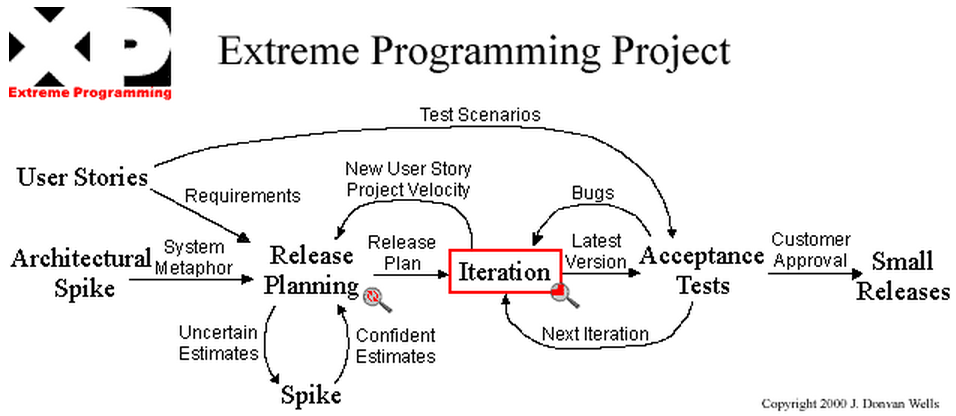
\includegraphics[width=12cm]{xp.png}
     \caption{XP:n prosessi~\cite{XP.ORGMAP}}\label{xprocess}
\end{figure}

\subsubsection{Kommunikointi}

Kasvokkaista ja usein tapahtuvaa kommunikointia painotetaan järjestämällä tiimin jäsenet yhteiseen tilaan. Tämän lisäksi projektia varten on hankittu vähintään yksi paikan päällä oleva asiakas, joka on osana kehitystiimiä nähdäkseen projektin edistymisen. Paikan päällä olevan asiakkaan kanssa keskustellaan kehityksen jokaisesta vaiheesta ja hän päättää sekä tuotteen vaatimuksista että niiden priorisoinnista. Asiakkaan läsnäolo on suuri etu, sillä tiimi voi kysyä häneltä hetkessä esimerkiksi jonkin toteutettavan vaatimuksen yksityiskohdista ja asiakas vastaavasti voi antaa heti palautetta työstä. Ryhmän sisäinen kommunikointi on suuressa osassa sillä hyvät ratkaisut saadaan useimmiten yhteistyön tuloksena. Kommunikoinnin ja yhteistyön merkitystä kuvastaa esimerkiksi \emph{pariohjelmointi} (pair 
programming), joka on yksi XP:n keskeisimpiä käytänteitä.

\subsubsection{Pariohjelmointi}

Pariohjelmoinnissa kaksi henkilöä ohjelmoivat pareittain, jakaen saman 
tietokoneen~\cite{Shore:2007:AAD:1407480}. Henkilöt eivät kuitenkaan ohjelmoi samaan aikaan, vaan 
heille on 
nimetty kaksi roolia: toinen on \emph{ajaja} (the driver), ja toinen 
\emph{navigoija} (the navigator). Ajajan tehtävänä on 
yksinkertaisesti 
kirjoittaa koodia. Navigoijan tehtävänä on analysoida jatkuvasti 
kirjoitettua koodia ja kertoa ajajalle mitä tehtäviä heidän tulee 
milloinkin 
toteuttaa. Näin ajaja voi keskittyä pelkästään ohjelmointiin. Sovituin 
väliajoin henkilöt vaihtavat rooleja. Pariohjelmointi voidaan nähdä 
ryhmätyöskentelynä --- kaksi ihmistä suorittavat yhteistä tehtävää 
saavuttaakseen saman päämäärän.\\

Pariohjelmointi korostaa yhteistyötä ja kommunikointia. Tästä on monia 
hyötyjä, jotka tekevät hyvää sekä ryhmän jäsenille, ryhmälle että 
projektille~\cite{Begel:2008:PPW:1414004.1414026}. Tarkastellaan näitä 
hyötyjä seuraavaksi. 

\begin{itemize}

\item {\bf Koodin laatu}

Kun kaksi henkilöä pariohjelmoivat ja ratkaisevat samaa ongelmaa, 
lopputulos on usein parempi verrattuna siihen, että yksi henkilö 
tekisi kaiken. Parit pystyvät helposti keskustelemaan keskenään siitä 
mitä heidän tulisi seuraavaksi tehdä ja he voivat jakaa ideoita 
saadakseen koodista laadukkaamman tai ratkaistakseen jonkin ongelman. 
Sivustakatsojana navigoija pystyy tekemään tärkeitä huomioita ja 
pohtimaan kuinka koodista saataisiin laadukkaampi, kun taas ajaja voi 
keskittyä ohjelmoimiseen. Navigoija tekee ajoittain ehdotuksia 
ajajalle, joilla koodista saataisiin parempaa.
Pariohjelmoinnin ansiosta tapahtuva laajamittaisempi koodin 
katselmointi vähentää virheiden määrää. Vaihtoehtoisesti
niitä ei edes synny, kun parit keskenään kommunikoivat miettien hyviä 
ratkaisuja.

Pariohjelmointi parantaa keskittymiskykyä. Toisen henkilön 
läsnäolo estää herkemmin yksilöä laiskottelemasta tai olla noudattamatta XP:n
vaalimia käytänteitä, kuten TDD:tä. Käytänteiden noudattaminen taas 
johtaa parempaan koodin laatuun ja toteutukseen.

\item {\bf Oppiminen}

Kun henkilöt toimivat pareittain toistensa kanssa, osaaminen 
leviää kehittäjien kesken. Monet tykkäävät neuvoa toisiaan ja ryhmän 
jäsenillä
on eri taitoja ja tietämystä asioista. Esimerkiksi ryhmän jäsenet, 
jotka pääsevät heitä taitavampien ihmisten pareiksi, voivat oppia
paljon uusia tekniikoita. Parhaimmassa tapauksessa koko ryhmän sisällä 
kaikki voivat oppia toisiltaan jotakin.
Oppimiseen sisältyy, että ymmärrys kehitettävästä ohjelmasta 
parantuu. Kun henkilöt vaihtavat
pareja eri ihmisten kanssa, he pääsevät näkemään erilaisia 
kehityksessä olevia ohjelman osia. Samalla he osallistuvat 
eri osien
kehitykseen, jolloin ymmärrys koko projektista kasvaa korkeammalle 
tasolle.\\

Pariohjelmointi on suuressa roolissa 
XP:ssä ja ryhmän jäsenien keskinäisellä vuorovaikutuksella on suuri 
hyöty projektin laadun kannalta. Pariohjelmoinnin 
hyvien puolien yhteisenä tekijänä on, että parit kommunikoivat 
toistensa kanssa. Ilman keskinäistä vuorovaikutusta ei voi odottaa, 
että edellä mainitut asiat toteutuisivat. Pariohjelmointi 
rohkaisee kehittäjiä puhumaan toisilleen, joten tästä ei pitäisi olla 
huolta~\cite{Zarb:2012:UCW:2384716.2384738}.

\end{itemize}

Seuraavaksi käsitellään XP:n prosessin eri vaiheet (ks. kuva \ref{xprocess}). Näistä vaiheista tullaan käsittelemään \emph{julkaisusuunnittelu} (release planning), \emph{iteraatio} (iteration) ja \emph{hyväksymätestaus} (acceptance testing).

\subsubsection{Julkaisusuunnittelu}

Kun asiakas on tehnyt listan vaatimuksia, joita kehitettävän järjestelmän pitää sisältää, siirrytään XP:n prosessissa \emph{julkaisusuunnitteluun} (release planning),
jossa on tarkoituksena tehdä julkaisusuunnittelun kokouksen aikana \emph{julkaisusuunnitelma} (release plan). XP:ssä on tapana iteraatioiden lopuksi julkaista uusin, toimiva versio asiakkaiden käyttöön. Julkaisusuunnitelma määrittelee, mitkä vaatimukset toteutetaan missäkin iteraatiossa. Iteraatioon valitut vaatimukset ovat valmiina iteraation lopuksi tehtävässä julkaisussa. Näille vaatimuksille määritellään päivämäärät.\\

Kokouksessa kehitystiimin tehtävänä on arvioida kuinka paljon yksittäinen vaatimus vie työaikaa. Arviointien perusteella asiakas
tekee päätök\-sen vaatimusten tärkeysjärjestyksestä. Tämän jälkeen tiimin jäsenet
yhdessä asiakkaan kanssa sijoittavat vaatimukset tietyille iteraatioille toteutettaviksi.

\subsubsection{Iteraatio}

Ennen kuin varsinainen iteraatio alkaa, jossa itse tuotteen tiettyjen toiminnallisuuksien
kehitys tapahtuu, järjestetään \emph{iteraatiosuunnittelun kokous} (iteration planning meeting), jossa tehdään \emph{iteraatiosuunnitelma} (iteration plan). Iteraatiosuunnittelun tavoitteena on päättää mitä iteraation aikana tehdään, joka kirjataan iteraatiosuunnitelmaan.

Suunnittelun alussa asiakas valitsee julkaisusuunnitelmasta korkeimman prioriteetin omaavat vaatimukset alkavaan iteraatioon. Kehittäjät pilkkovat nämä vaatimukset pieniksi, toteutettaviksi tehtäviksi. Tämän jälkeen kehittäjät päättävät ketkä toteuttavat minkäkin tehtävän ja he estimoivat tehtäviin kuluvan työmäärän. Lopuksi vaatimukset, tehtävät ja niiden estimaatit kirjataan iteraatiosuunnitelmaan.\\

Iteraatiosuunnittelun ja onnistuneen suunnitelman tekemisen jälkeen voidaan aloittaa itse iteraatio. Iteraatio kestää 1-4 viikkoa, jonka aikana iteraatiosuunnitelmaan kirjatut vaatimukset ja niihin liittyvät tehtävät pitää toteuttaa. Kehitystyö tapahtuu pariohjelmoiden, jonka
merkitystä ryhmätyöskentelyyn aikaisemmin tarkasteltiin. Iteraatioon liittyy päivittäinen palaveri, jossa ryhmän jäsenet raportoivat toisilleen mitä saivat viime palaverin jälkeen aikaan, mitä aikovat saada aikaan ennen seuraavaa palaveria ja onko heidän etenemisessään ongelmia. Näin tiimin jäsenet ovat jatkuvasti tietoisia
muiden jäsenten sekä koko tiimin tilanteesta. Kuten edellä on mainittu, iteraation aikana on vähintään yksi asiakas läsnä joka päivä, jonka kanssa voi puhua ongelmatilanteissa toteutettavien vaatimusten yksityiskohdista ja neuvotella kehityksestä.\\

Iteraation lopuksi suoritetaan \emph{hyväksymätestaus} (acceptance testing), jossa testataan iteraation aikana toteutettuja vaatimuksia ja varmistutaan siitä, että ne toimivat oikein. Asiakas on määritellyt tarkemmin mitä skenaarioita testien tulisi testata. Jos yksittäinen vaatimus läpäisee kaikki siihen kohdistuvat testit, on vaatimus toteutettu valmiiksi. Asiakas itse tarkistaa testitulokset ja päättää niiden perusteella onko viimeisin versio tuotteesta julkaisukelpoinen. Jos testauksen aikana löytyy ohjelmointivirheitä, ne kirjataan ylös ja korjataan seuraavan iteraation aikana.\\

Ketteränä menetelmänä XP on iteratiivinen, joten kun yksi iteraatio on loppunut, aloitetaan edellä mainittu prosessi uudestaan alkaen julkaisusuunnittelun kokouksella. XP:n prosessia jatketaan, kunnes tuote on valmis. XP painottaa hyvin paljon asiakkaan kanssa kommunikointia ja läsnäoloa, jotta kehityksessä ei päädytä sivuraiteille. Asiakas on osana ryhmää ja hänen kanssaan tapahtuva kommunikointi ja yhteistyö vaikuttaa projektin onnistumiseen yhdessä ryhmän sisäisen kommunikoinnin kanssa.

\subsection{Scrum}

\begin{figure}[ht]
     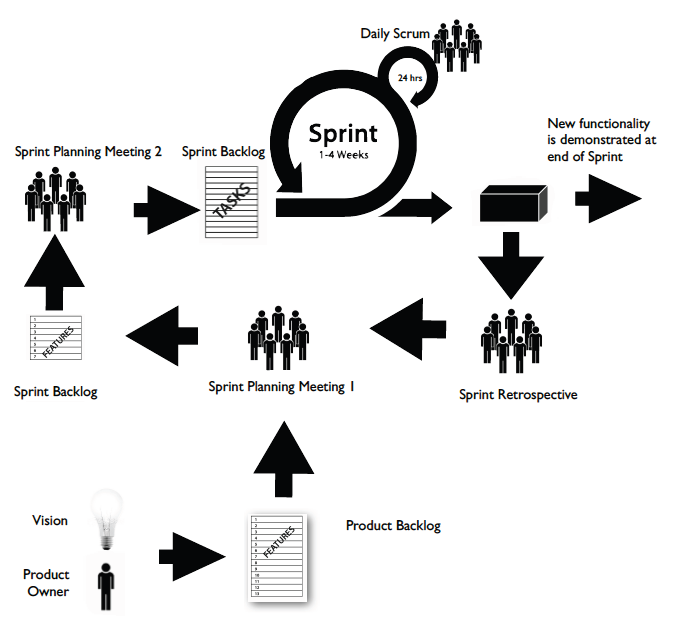
\includegraphics{scrum.png}
     \caption{Scrumin prosessi~\cite{Scrumprimer}}\label{scrumprocess}
\end{figure}

Scrum on prosessimalli, joka painottaa tiimien yhteistyötä projektin 
kehityksessä~\cite{ScrumORG}. Scrum, kuten XP, on iteratiivinen 
ja inkrementaalinen menetelmä.
Kehitys tapahtuu lyhyissä 1-4 viikon sykleissä, 
\emph{"sprinteissä"}, joissa toteutetaan kehitettävää tuotetta tietyt 
toiminnallisuudet kerrallaan. Lyhyet kehityssyklit sallivat tiimien 
mukautuvan asiakkaalta saatavaan palautteeseen ja vaatimusten 
muutoksiin. Näin tuotteeseen voidaan tehdä ajoissa
muutoksia ilman suuria kuluja ja tuote "hioutuu"~yhä lähemmäs sitä 
mitä asiakas sen haluaa olevan. Scrum tekee projektin kehityksestä
monivaiheisen, kuten kuvassa \ref{scrumprocess} näkyy. Vaiheet käsitellään tässä luvussa. Seuraavissa osioissa kerrotaan millainen Scrum-tiimi
on ja millainen projektin elinkaari on Scrumissa.

\subsubsection{Tiimi}

Scrumissa tiimit koostuvat \emph{monitaitoisista} (cross-functional) 
jäsenistä, joilta löytyy tarpeellinen tekninen osaaminen, jota 
vaaditaan
tuotteen toteuttamiseen. Tiimillä ei ole johtajaa tai 
projektipäällikköä, jotka määräisivät tiimin tekemisistä. Sen sijaan tiimillä on henkilö, jonka rooli on \emph{"Scrum master"}. Scrum masterin tehtävänä on valvoa, että tiimi noudattaa Scrumin prosessia ja hän pitää huolen, että ulkopuoliset henkilöt eivät tule häiritsemään tiimiä.
Tiimi saa itse päättää tavoitteet joka sprintille ja sen miten nämä tavoitteet 
saavutetaan. Toisin sanoen tiimi on \emph{itseorganisoituva}
(self-organizing). Tämä on Scrumille olennaista ja siitä näkee 
kuinka suuressa arvossa tiimin jäsenten välistä yhteistyötä 
pidetään~\cite{ScrumHandBook}.

\subsubsection{Scrumin aloitus}

Scrumin ensimmäinen askel on luoda lista tuotteen vaatimista
ei-toiminnalli\-sista ja toiminnallisista vaatimuksista. Vaatimukset
kootaan listaksi, jota kutsutaan \emph{tuotteen kehitysjonoksi} (product backlog)~\cite{ScrumFinnishGuide}. Kehitysjono on priorisoitu siten, että tärkeimmät vaatimukset ovat kehitysjonon kärjessä. Kehitysjono on jatkuvan muutoksen alaisena: uusia vaatimuksia
voi tulla lisää asiakkaan toimesta, tarpeettomia vaatimuksia karsitaan ja olemassaolevia muokataan tai tarkennetaan. Edellä mainitut tehtävät
ovat niin kutsutun \emph{tuoteomistajan} (product owner) vastuulla,
joka on yksittäinen henkilö ja pitää huolen tuotteen arvon ja kehitystiimin työn arvon maksimoimisesta. Tuoteomistaja voi pyytää kehitystiimiä auttamaan edellä mainituissa tehtävissä.

\subsubsection{Sprintin suunnittelupalaveri}

Jokaisen sprintin aluksi järjestetään kokous, jota kutsutaan \emph{sprintin suunnittelupalaveriksi} (sprint planning meeting)~\cite{ScrumHandBook}. Palaveri on kaksiosainen.
Ensimmäisessä osassa tuoteomistaja ja kehitystiimi neuvottelevat
siitä mitkä vaatimukset tiimin tulisi toteuttaa alkavassa
sprintissä. Päätösvastuu on tiimin jäsenillä.\\

Toisessa osassa tiimi valitsee toteutettavat vaatimukset, jotka
he sitoutuvat tekemään sprintin loppuun mennessä. Vaatimukset
valitaan aina kehitysjonon kärjestä.
Kun vaatimukset on valittu, ne pilkotaan pienemmiksi, teknisiksi
tehtäviksi, joille arvioidaan niihin kuluva aika. Nämä tehtävät kirjataan aika-arvioineen \emph{sprintin tehtävälistaan} (sprint backlog), jota tiimi käyttää hyödykseen sprintin ajan. Tiimi saa itse valita toteutettavat vaatimukset alkavalle sprintille sekä suunnitella miten ne toteutetaan.

\subsubsection{Scrumin päiväpalaveri}

Kun sprintti alkaa, sen aikana harjoitetaan jokapäiväistä Scrumin käytäntöä:
\emph{päiväpalaveria} (daily Scrum). Tämä on lyhyt, noin 15 minuuttia kestävä kokoontuminen, johon
kaikki tiimin jäsenet osallistuvat. Jokainen tiimin jäsen raportoi kolme asiaa muille tiimin jäsenille:
mitä henkilö on saanut aikaan viime tapaamisen jälkeen, mitä henkilö
aikoo saada aikaan ennen seuraavaa tapaamista ja onko mitään
esteitä työn etenemiselle. Näin tiimin jäsenet säännöllisesti tietävät
kuinka muiden työ edistyy ja palaverin jälkeen mahdollisia raportoituja
ongelmia voidaan yhdessä ratkoa. Huomionarvoista on, että päiväpalaveriin ei mieluiten osallistu esimiehiä tai muita
ulkopuolisia henkilöitä~\cite{ScrumHandBook}. Jos näin käy, on riski,
että henkilöt tuntevat olevansa tarkkailun alaisena, mikä voi
tuottaa heille paineita oman edistymisen tai ongelmien raportoinnista.

\subsubsection{Sprintin katselmointi}

Sprintin lopussa järjestetään \emph{sprintin katselmointi} (sprint review), jossa tiimi esittelee sprintin aikana toteuttamiaan
vaatimuksia tuoteomistajalle ja asiakkaalle. Asiakas ja tuoteomistaja
tietävät näin miten projekti on edistynyt ja tiimi vastaavasti saa
arvokasta palautetta. Annettu palaute kirjataan mahdollisina muutoksina
vaatimuksiin tai uusina vaatimuksina tuotteen kehitysjonoon.

\subsubsection{Sprintin retrospektiivi}

Viimeisenä asiana sprintin lopuksi järjestetään \emph{sprintin retrospektiivi}
(sprint retrospective), jossa tiimi keskustelee kuinka heidän
oma työprosessinsa sujui sprintin aikana~\cite{Scrumprimer}. Jäsenet
keskustelevat yhdessä mikä sprintissä sujui hyvin ja missä
asioissa pitäisi parantaa. Jäsenien antama palaute ja kritiikki
voi esimerkiksi kohdistua yksittäisen jäsenen työskentelytapoihin.
Jos mahdollisia ongelmakohtia on, tiimin tulisi yhdessä päättää
miten ongelmat ratkaistaan. Retrospektiivi on tärkeä vaihe
ryhmätyöskentelyn kannalta, koska se on Scrumin pääasiallisin
mekanismi tuoda tiimin ongelmat näkyville ja ratkaista ne siten,
että ryhmän työskentely vahvistuu ja paranee.\\

Kun edellä mainitut vaiheet on käyty läpi, alkaa uusi
sprintti. Käytännössä aloitetaan uusi sykli aloittaen
sprintin suunnittelupalaverista. Tätä periaatteessa jatketaan
niin kauan, kunnes tuote on valmis eli asiakkaan kaikki vaatimukset
on toteutettu. Kuten kävi ilmi, kehitystiimin jäsenillä on paljon valtaa sen suhteen mitä he tekevät ja miten he
sen tekevät. Suunnittelutyö ja toteutus ovat asioita, jotka tiimin
jäsenet yhteisymmärryksessä päättävät kommunikoiden toistensa kanssa.

\section{Persoonallisuuden vaikutus}

Kehitystiimit koostuvat erilaisista ihmisistä. Useissa tutkimuksissa on huomattu, että tietyt
luonteenpiirteet ja persoonallisuustyypit vaikuttavat positiivisesti tiimin suorituskykyyn sekä
projektin onnistumiseen~\cite{Acuna:2008:ESP:1414004.1414056,Capretz:2003:PTS:766407.766410,Capretz:2010:MSS:1726559.1726574,Gorla:2004:WWB:990680.990684}. Sen lisäksi, että tiimien on hyvä koostua monitaitoisista
jäsenistä, moninaiset persoonallisuustyypit tiimin sisällä ovat hyväksi
projektille. Esimerkiksi suurempia ratkaisuja mietittäessä harvoin hyväksytään
ensimmäinen ehdotus, joka esitetään, vaan puntaroidaan monen ehdotuksen
välillä arvioiden niiden hyviä ja huonoja puolia. Myös yksilön oma
tekninen osaaminen vaikuttaa ratkaisun miettimiseen. Eri tavalla ajattelevat ihmiset kykenevät tuomaan joukon
eri näkökulmia tuotetta kehitettäessä, jotka johtavat parempiin ratkaisuihin.\\

Edellä mainitun lisäksi henkilön persoonallisuus vaikuttaa
kuinka mieluista kyseisen henkilön kanssa on työskennellä,
miten henkilö lähestyy annettua tehtävää ja minkälaisiin tehtäviin
hän soveltuu parhaiten~\cite{Begel:2008:PPW:1414004.1414026,Capretz:2010:MSS:1726559.1726574}. Yksi tapa mitata henkilön persoonallisuutta on käyttää Myers-Briggsin tyyppi-indikaattoria.
Seuraavissa osioissa tarkastellaan millaisia piirteitä hyvällä
ohjelmistokehittäjällä on ja mitkä erilaiset persoonallisuustyypit
sopivat parhaiten projektien eri kehitysvaiheisiin. Ennen tätä kuitenkin kerrotaan millainen Myers-Briggsin tyyppi-indikaattori on, jonka avulla pohjustetaan tulevia osioita.

\subsection{Myers-Briggsin tyyppi-indikaattori}

Persoonallisuustyyppejä määriteltäessä voidaan käyttää apuna
Myers-Briggsin tyyppi-indikaattoria, joka jakaa ihmisen persoonallisuuden neljään eri osioon: sosiaaliseen vuorovaikutukseen, tiedonkeruuseen, päätöksentekoon ja elämän\-tyyliin~\cite{Capretz:2003:PTS:766407.766410,Capretz:2010:MSS:1726559.1726574,DaCunha:2007:PMA:1230819.1241672}. Joka osiossa on
kaksi eri luonteenpiirrettä. Kussakin osiossa jokainen ihminen kallistuu enemmän toiseen piirteeseen kuin toiseen eli Myers-Briggsin
tyyppi-indikaattorilla saadaan yksittäiselle henkilölle näistä osioista neljä luonteenpiirrettä, jotka määrittävät hänen persoonallisuuden. Yhteensä
persoonallisuustyyppejä on $2^4$ = 16 erilaista.

\begin{enumerate}

\item Sosiaalinen vuorovaikutus: Ekstrovertti (E) --- Introvertti (I)

Ekstrovertit ovat sosiaalisia, ulospäinsuuntautuneita ja nauttivat
muiden ihmisten seurasta. Introvertit sen sijaan ovat sisäänpäinkääntyneitä, hiljaisia, varautuneita ja ovat mieluummin omissa oloissaan.

\item Tiedonkeruu: Tosiasiallinen (S) --- Intuitiivinen (N)

Tosiasialliset ihmiset etsivät yksityiskohtaista tietoa ja tunnettuja
tosiasioita. He uskovat enemmän konkreettisiin asioihin, jotka
voivat itse todistaa. Intuitiiviset etsivät asioille
yhteyksiä teoreettisemman tiedon pohjalta ja
he miettivät eri asioista aiheutuvia mahdollisuuksia.

\item Päätöksenteko: Ajatteleva (T) --- Tunteva (F)

Ajattelevat perustavat päätöksensä miettimällä tarkasti päätöksen syitä, seurauksia ja loogisuutta. He perustavat päätöksensä järjen käyttöön. Tuntevilla on taipumus tehdä päätös
henkilökohtaisten arvojen perusteella sekä sen mukaan miten päätös
vaikuttaa muihin ihmisiin. Päätöksenteko vaikuttaa siihen minkälaisista tehtävistä
henkilö kiinnostuu ja kuinka tyytyväinen hän on niihin.

\item Elämäntyyli: Järjestelmällinen (J) --- Spontaani (P)

Järjestelmälliset ihmiset ovat sananmukaisesti järjestelmällisiä
ja täsmäl\-lisiä. He pitävät aikamääreistä kiinni ja suunnittelevat
asioita etukäteen. Spontaanit taas ovat joustavia ja elävät
hetkessä välittämättä suunnitelmallisuudesta ja järjestelmällisyydestä.
Elämäntyyli vaikuttaa henkilön työskentelytapoihin.

\end{enumerate}

\subsection{Ohjelmistokehittäjän piirteet}

Usein todetaan, että hyvälle ohjelmistokehittäjälle on aina tilaa ohjelmistoalalla.
Siinä missä tekninen osaaminen ja hyvä tietämys asioista on
tärkeää, ihmistaidot ja kommunikointi on saanut
huomiota alalla~\cite{Hall:2007:CNT:1235000.1235043}. Esimerkiksi
pariohjelmoinnissa työskentely vaatii kommunikointia ja sitä, että
tulee toisten ihmisten kanssa toimeen. Hyvä ohjelmistokehittäjä
on mieluinen työkumppani. Vastakohtana ohjelmistoalalla
on väistämättä huonoja ohjelmistokehittäjiä, jotka tekevät
yhteistyöstä epämiellyttävää.\\

Seuraavaksi tarkastellaan ohjelmistokehittäjän hyviä ja huonoja
piirteitä. Hyvissä piirteissä painotus on ominaisuuksissa, jotka
tekevät kehittäjästä mieluisan työkumppanin hyvien teknisten
taitojen lisäksi. Samalla tavalla huonoissa piirteissä tarkastellaan
enimmäkseen ominaisuuksia, jotka tekevät kehittäjästä epämieluisan työkumppanin. Tekninen osaaminen on sivuroolissa.\\

Tutkimuksissa
on haastateltu ohjelmistoalan ammattilaisia ja kysytty heiltä mitkä
piirteet tekevät hyvän ohjelmistokehittäjän~\cite{Acuna:2008:ESP:1414004.1414056,Begel:2008:PPW:1414004.1414026,Hall:2007:CNT:1235000.1235043}. Haastattelujen perusteella seuraavat piirteet ovat tärkeimpiä:

\begin{itemize}

\item {\bf Joustava \& mukautuva}

Joustava henkilö on avaramielinen. Henkilö kuuntelee mielellään muiden
ideoita ja kykenee katsomaan asioita eri näkökulmista sen sijaan, että
puolustelisi vain omaa kantaansa. Hän on halukas yhteistyöhön
ja pystyy mukautumaan eri työtapoihin.

\item {\bf Hyvät kommunikointitaidot}

Ohjelmiston kehittäminen vaatii paljon ryhmätyöskentelyä ja
kommunikointia tiimin jäsenten kesken. Hyvä kommunikoija kykenee
kuuntelemaan muiden ideoita, ilmaisee omat mielipiteensä selkeästi ja uskaltaa
kysyä apua, jos hänellä on ongelmia. Kun tiimi koostuu jäsenistä,
jotka kommunikoivat usein ja hyvin, se vaikuttaa positiivisesti
ilmapiiriin ja työn laatuun. Kommunikoinnin myötä
tieto leviää tiimin jäsenten kesken, joka kasvattaa kaikkien osaamista.

\item {\bf Älykäs}

Ohjelmistokehitys on teknistä työtä, joten
ihmistaitojen lisäksi myös älykkyys on erittäin tärkeä piirre.
Älykkyydellä tarkoitetaan tässä tapauksessa sellaista ohjelmistokehittäjää, jolla on hyvä tekninen osaaminen ja, joka on nopea
ajatuksissaan. Henkilön ongelmanratkaisutaidot ovat erinomaiset
ja hän kykenee ajattelemaan asioita abstraktilla tasolla sekä ottaa
vastuuta työstään.

\item {\bf Mukava}

Mukava ohjelmistokehittäjä on sosiaalinen ja hänen kanssaan on
helppo työskennellä. Hänellä on huumorintajua ja sopivaa
tilannetajua eli esimerkiksi pystyy huomauttamaan virheistä ilman,
että toinen pahastuu. Lyhyesti sanottuna kyseisen henkilön kanssa
on hauska työskennellä.

\end{itemize}

Muita hyviä piirteitä ovat muun muassa, että ohjelmistokehittäjä
on tietäväinen, innovatiivinen, itsenäinen, kykenee keskittymään työhönsä, ja noudattaa käytettyä prosessia.\\

Huonot ohjelmistokehittäjät eivät ole haluttavia ryhmän jäseniä tai
työkumppaneita. Hallin ja kumppaneiden haastatteluissa kysyttiin millaisia ovat huonot kehittäjät~\cite{Hall:2007:CNT:1235000.1235043}. Tuloksena oli, että huono ohjelmistokehittäjä on tekniseltä osaamiseltaan heikko ja hänellä on huonot kommunikointitaidot. Huonoilla kommunikointitaidoilla haastateltavat tarkoittivat seuraavia asioita:

\begin{enumerate}

\item Ei raportoi ongelmista.
\item On haluton kuuntelemaan muiden ideoita.
\item On itsepäinen.
\item Ei kunnioita muiden asemia.

\end{enumerate}

Kun tähän lisätään hyvien piirteiden vastakohtia, on huono kehittäjä huumorintajuton, ei ota työstään vastuuta ja hänellä on vaikeuksia omaksua uusia työtapoja tai rooleja. Tekniseltä osaamiseltaan kehittäjän ongelmanratkaisutaidot ovat heikot eikä hänellä ole kykyä ajatella asioita abstraktisti.\\

Mainitsemisen arvoisia ovat Pietersen ja kumppaneiden kertomista yksittäisen henkilön osallistumisen tasoista ryhmätyös\-kentelyssä~\cite{Pieterse:2012:PPS:2157136.2157218}.
Huono kehittäjä ei luota muiden apuun ja haluaa tehdä asioita yksin. Kehittäjä näkee muut ryhmän jäsenet epäpätevinä ja hänen asenteensa mahdollisesti lannistaa muiden ryhmän jäsenten motivaatiota. Toisenlainen huono kehittäjä taas tekee vähemmän työtä kuin mitä häneltä odotetaan.
Pietersen ja kumppaneiden tekemässä ryhmätyöhön liittyvässä kokeilussa havaittiin, että ryhmistä löytyi jäseniä, jotka vastasivat edellä mainittuja huonoja ryhmän jäseniä.

\subsection{Persoonallisuustyypit eri kehityksen vaiheissa}

Ohjelmistokehitys on monivaiheinen prosessi, joka on perinteisessä ohjelmistotuotannossa
jaettu vaatimusmäärittelyyn, suunnitteluun, toteutukseen, testaukseen
ja ylläpitoon. Nämä eri vaiheet vaativat erilaisia teknisiä taitoja,
jotta saadaan paras mahdollinen lopputulos. Teknisen
osaamisen lisäksi myös persoonallisuustyyppi vaikuttaa siihen kuinka
hyvin henkilö suoriutuu tietyistä tehtävistä tai kuinka hyvin hän
soveltuu niihin~\cite{Capretz:2010:MSS:1726559.1726574}. Kun luonteiltaan oikeanlaiset henkilöt valitaan suorittamaan
näitä tiettyjä kehityksen vaiheita, tuloksena on parempi lopputulos
projektin kannalta.\\

Seuraavaksi käydään edellä mainitut kehityksen vaiheet läpi yksi kerrallaan
sekä tarkastellaan millaiset ohjelmistokehittäjät sopivat
parhaiten mihinkin vaiheeseen. Oletetaan, että kehittäjillä on
hyvä tekninen osaaminen kaikissa vaiheissa, jolloin tarkastelu
voidaan rajoittaa ainoastaan siihen kuinka hyvin he persoonallisuustyypeiltään soveltuvat suorittamaan tiettyjä
kehityksen vaiheita.

\subsubsection{Vaatimusmäärittely}

Perinteisesti ohjelmistotuotanto alkaa vaatimusmäärittelyllä~\cite{SWEBOK:409902,Sommerville:2005:IRE:1042197.1042341}. Tämän vaiheen tavoitteena on selvittää mitä vaatimuksia
tuotteella eli valmiilla ohjelmalla on. Vaatimuksilla voidaan tarkoittaa toiminnallisia vaatimuksia eli
mitä ohjelma tekee tai mitä sillä pystytään tekemään, tai ei-toiminnallisia vaatimuksia eli esimerkiksi millä kielellä
ohjelma kirjoitetaan, kuinka käytettävä tai tehokas sen tulee olla ja niin edelleen.\\

Vaatimusmäärittely tehdään usein asiakkaan kanssa, jolla on etukäteen jonkinlainen kokonaiskuva valmiista ohjelmasta.
Kehittäjien täytyy keskustella asiakkaan kanssa saadakseen selville millaisesta ohjelmasta on kyse ja mitä sen tulisi tehdä.
Vaatimusmäärittelyssä tulee kartoittaa ensinnäkin keitä ovat ohjelman käyttäjät ja millaisia käyttötilanteita
käyttäjillä on ohjelmaan liittyen. Asiakkaan kanssa luodaan lopuksi lista vaatimuksia toteutettavalle ohjelmalle,
jotka seuraavaksi analysoidaan. Analysoinnilla tutkitaan ovatko vaatimukset tarpeeksi kattavat eli määrittävätkö ne asiakkaan
haluaman tuotteen sekä tarkistetaan, että vaatimukset eivät ole ristiriidassa toistensa kanssa. Jos vaatimukset vaikuttavat
kattavilta ja ristiriidattomilta, niin lopuksi vielä varmistetaan asiakkaalta, että vaatimukset ovat hänen mieleensä ja
edustavat sitä mielikuvaa tuotteesta, joka hänellä on.
Lopuksi vaatimukset dokumentoidaan, jotta kehittäjät tietävät ja muistavat jatkossakin mitä heidän tulee toteuttaa sekä testata.\\

Capretz ja Ahmed ovat tutkineet millainen kehittäjä soveltuu
parhaiten järjestelmäanalyysiin, joka on sidoksissa vaatimusmäärittelyyn~\cite{Capretz:2010:MSS:1726559.1726574}.
Järjestelmä\-analyysiin tarvitaan kehittäjiä, jotka ymmärtävät asiakkaan tarpeet ja käsittävät mitkä ovat ohjelman keskeisimmät toiminnot.
Järjestelmäa\-nalyysi vaatii paljon kommunikointia asiakkaan kanssa,
joten ekstrovertit (E) soveltuvat tähän hyvin, koska he ovat parempia
puhumaan ja saamaan asiakkaasta vastauksia irti toisin kuin introvertit (I), jotka eivät ole yhtä hyviä ilmaisemaan asioita selkeästi. 
Kehittäjän tulee myös asettua käyttäjän rooliin ja miettiä
käyttäjän tarpeita. Tähän tarpeeseen on tuntevat (F) ihmiset hyviä. Vaatimusmäärittelyssä keskustellaan samaan tapaan asiakkaan kanssa, jossa tämän kaltaiset henkilöt ovat tarpeellisia. Optimaalisinta olisi määrätä vaatimusmäärittelyyn kehittäjiä, jotka ovat sekä ekstrovertteja että tuntevia (EF).\\

Gorlan ja Lamin mielipiteet eroavat edellä mainitusta~\cite{Gorla:2004:WWB:990680.990684}. Heidän mukaan ajattelevat (T) kehittäjät ovat tuntevia (F) parempia tässä työssä, jos kyse on pienestä tiimistä. Pienemmissä tiimeissä vaatimusten määrittelyn lisäksi kehittäjä voi joutua tekemään paljon muutakin, kuten suunnittelua ja ohjelmointia, jolloin analyyttinen ajattelutapa on parempi.

\subsubsection{Suunnittelu}

Suunnittelu on prosessi, jossa määritellään ohjelman arkkitehtuuri, komponentit, rajapinnat sekä muut ohjelmaan liittyvät osat~\cite{SWEBOK:409902}.
Suunnittelussa hahmotellaan vaatimusten perusteella mistä komponenteista ja pienemmistä osasista järjestelmä koostuu, ja mitkä ovat niiden tehtävät. Suunnittelussa mietitään miten järjestelmän eri osat ovat vuorovaikutuksessa toistensa kanssa, millaiset rajapinnat niillä on ja mitä palveluita ne tarvitsevat muilta järjestelmän osilta.
Tarkoituksena on luoda ohjelmasta malli, joka toteuttaa kirjatut vaatimukset, ja jonka voi muuttaa ohjelmakoodiksi.\\

Suunnittelu on luovaa ja tutkivaa työtä, jossa suunnittelija miettii mitkä ovat järjestelmän avainkomponentit, ja hahmottelee parhaita ratkaisuja erilaisten käyttötilanteiden avulla. Suunnittelijalla tulisi olla kokonaiskuva järjestelmästä ja kyky erotella relevantit asiat annetusta datasta, kuten vaatimuksista. Tämä vaatii intuitiota.
Suunnittelijoiden tulisi siis olla intuitiivisia (N), koska tällaiset henkilöt ovat luovia ja kokeilevat erilaisista asioista tapahtuvien mahdollisuuksien yhdistelyä. Hyvän tuloksen saamiseksi tarvitaan ongelmanratkaisutaitoja, joita ajattelevilla (T) on. On suositeltavaa, että suunnittelija on sekä intuitiivinen että ajatteleva (NT)~\cite{Capretz:2010:MSS:1726559.1726574}.

\subsubsection{Toteutus}

Kun suunnittelu on ohi, siirrytään toteutukseen~\cite{SWEBOK:409902}. Suunnitteluvaiheessa ohjelmasta ollaan luotu korkean tason malli, joka kertoo millaisista komponenteista ohjelma koostuu
ja mitkä ovat eri komponenttien tehtävät. Toteutuksessa muunnetaan malli ohjelmakoodiksi ja siten konkreettiseksi ohjelmaksi.\\

Toteutus on suurimmaksi osaksi ohjelmointia, johon liittyy suunnittelua ja testausta. Ohjelmoijan tulee tunnistaa ohjelman
osille tärkeät muuttujat, rakenteet ja tietorakenteet. Ohjelmoijan
tulee luonnollisesti hallita ohjelmointikieli, jolla ohjelma kirjoitetaan. Siinä missä ohjelmalle tehty malli voi olla hyvinkin korkeatasoinen, koodin kirjoittaminen vaatii paneutumista yksityiskohtiin ja mallin sekä vaatimusten muuntaminen suoraviivaiseksi koodiksi vaatii loogista ajattelutapaa. Ajatteleva (T)
henkilö soveltuu loogiseen ajatteluun paremmin kuin tunteva (F). Lisäksi yksityiskohtiin ja faktatietoihin paneutuminen on tosiasiallisen (S) ihmisen aluetta enemmän kuin intuitiivisen (N). Vaikka aiemmin on todettu kehityksen vaativan ryhmätyötä ja kommunikointia, Capretz ja Ahmed näkevät ohjelmoinnin teknisenä työnä, joka loppupeleissä vaatii itsenäistä työskentelyä ja keskittymiskykyä enemmän kuin ryhmätyöskentelyä. Täten introvertit (I) sopivat ohjelmoijiksi ekstrovertteja (E) paremmin. Ihanteellinen yhdistelmä ohjelmoijalle olisi, että hän on introvertti, tosiasiallinen ja ajatteleva (IST). Tätä väitettä tukee se, että monien tutkimusten mukaan useimmat ohjelmistokehittäjät ovat persoonallisuustyyppiä ISTJ~\cite{Capretz:2003:PTS:766407.766410,Capretz:2010:MSS:1726559.1726574}.\\

Gorlan ja Lamin havainnot poikkeavat ideaalista ohjelmoijasta, kun kyse on pienistä tiimeistä~\cite{Gorla:2004:WWB:990680.990684}. Tiimin suorituskyky on parempi, jos ohjelmoijat ovat ekstrovertteja (E). Pienissä tiimeissä ohjelmoijien pitää kommunikoida eri osapuolten kanssa, kuten muiden tiimin jäsenten kanssa. Lisäksi pienissä tiimeissä ohjelmoija voi joutua tekemään monia muitakin tehtäviä kuin vain ohjelmointia, kuten ohjelman suunnittelua ja kommunikointia asiakkaan tai käyttäjien kanssa. Tällöin ekstroverttius on eduksi.
\looseness=-1

\subsubsection{Testaus}

Testausvaiheessa on tarkoituksena tehdä testejä, joilla varmistetaan ohjelman toimivuus~\cite{SWEBOK:409902}. Vaatimukset ovat ensisijaisia
testauskohteita eli testien avulla tarkistetaan, että ohjelmalle asetetut vaatimukset, jotka ovat toteutettu, toimivat
moitteettomasti. Testauksella pyritään myös löytämään ohjelmasta mahdollisimman paljon virheitä tekemällä testitilanteita, joissa yritetään
tehdä jotain luvatonta toimintaa, jota ohjelman ei tulisi sallia. Esimerkiksi, jos ohjelma on yksinkertainen laskin,
joka pyytää syöttämään yhteenlaskua varten kaksi lukua ja käyttäjä yrittää syöttää kirjaimista koostuvan merkkijonon, ohjelman
tulee osata varautua tähän ilman, että se hajoaa.\\

Testauksella on monta eri tasoa, joita ovat muun muassa yksikkötestaus,
integrointitestaus ja järjestelmätestaus~\cite{Capretz:2010:MSS:1726559.1726574}.
Yksikkötestauksessa testataan ohjelman komponentteja, luokkia
ja metodeita. Integraatiotestauksessa varmistetaan, että nämä komponentit, luokat ja metodit toimivat niiden ollessa keskinäisessä vuorovaikutuksessa, pyytäen ja tarjoten palveluita toisilleen. Järjestelmätestauksessa ohjelmaa testataan sen tarjoaman rajapinnan kuten käyttöliittymän kautta. Järjestelmätestaus liittyy vaatimuksiin, jotka määrittävät, että järjestelmällä pitäisi pystyä tekemään jotain ja järjestelmän tulisi vastata tähän toimintoon vaatimusten mukaisesti.\\

Testaukseen on monenlaisia strategioita, jotka noudattavat järjestelmälli\-siä lähestymistapoja. Testaus vaatii paneutumista yksityiskohtiin, jotta testaaja varmasti tarkistaa, että pienimmätkin ohjelman osat toimivat oikein. Tarkkuus ja järjestelmällisyys ovat
haluttavia ominaisuuksia testaajalle, joita tosiasialliset (S) ja järjestelmälliset (J) henkilöt edustavat. Menestyvät testaajat olisivat sekä tosiasiallisia että järjestelmällisiä (SJ)~\cite{Capretz:2010:MSS:1726559.1726574}.

\subsubsection{Ylläpito}

Ennen ylläpitoa ohjelma on julkaistu kohderyhmän käyttöön valmiina tuotteena, joka toteuttaa vaatimukset~\cite{SWEBOK:409902}. Ylläpidon
tarkoituksena on parannella tai muokata ohjelmaa, jolla tarkoitetaan lähinnä ohjelmointivirheiden
korjaamista ja optimointia. Ylläpidossa saatetaan lisätä myös aivan uusia toiminnallisuuksia
ohjelmaan. Kaiken tämän tarkoituksena on pidentää ohjelman käyttöikää sekä varmistaa käyttäjien
tyytyväisyys.\\

Ohjelman ylläpitäminen ja parantelu sopii tosiasiallisille (S) kehittäjille, koska he suosivat tuttujen tehtävien tekoa, jotka eivät vaadi uusien asioiden kokeilua. Intuitiiviset (N) sen sijaan haluavat kokeilla jotain uutta ja luultavasti tylsistyisivät ylläpitoon, jossa tehdään jonkinlaisia parannuksia ja pieniä ohjelmointivirheiden korjauksia. Tosiasialliset suosivat töitä, joissa aiemmin opitun tiedon käyttö on riittävää tehtävän suorittamiseen sen sijaan, että tulisi keksiä uusia ratkaisuja. He myös osaavat keskittyä yksityiskohtiin ja haluavat tietää miten asiat toimivat, joten heillä on hyvä kokonaiskuva järjestelmästä, jota ylläpitäminen vaatii. Spontaanit (P) sopeutuvat muutoksiin, jolloin heitä ei haittaisi järjestelmän jatkuva muokkaaminen. Tosiasialliset ja spontaanit kehittäjät ovat hyviä ylläpitäjiä (SP)~\cite{Capretz:2010:MSS:1726559.1726574}.\\

Edellä mainitut vaiheet ovat kaikki oleellisia ketterissä menetelmissä. Ketterät menetelmät perustuvat iteratiiviseen ja inkrementaaliseen kehitysmalliin, jonka ideana on tehdä ohjelmisto sykleissä, joissa ohjelmistosta tuotetaan vain osa. Tämä osa tuotetaan valmiiksi niin, että sykli sisältää vaatimusmäärittelyn, suunnittelun, toteutuksen, testauksen ja ylläpidon. Käytännössä tämä tarkoittaa, että yhden syklin aikana sama tiimi työstää yhdessä näitä vaiheita eli tiimin jäseniä ei eroteta ottamaan vastuuta vain tietystä vaiheesta. Kuten on todettu, monipuolinen tiimi eri persoonallisuuksilla täytettynä tuottaa paljon eri näkökulmia ja ratkaisuja. Persoonallisuutta katsottaessa yksittäinen henkilö saattaa olla toista henkilöä parempi tietyssä kehityksen vaiheessa, joten ketterissä menetelmissä on hyvä olla tiimi, jonka jäsenet ovat erilaisia luonteiltaan.

\section{Ryhmätyötaitojen parantaminen}

Hyvät ryhmätyö- ja kommunikointitaidot eivät ole itsestäänselvyys. Tietojenkäsittelytieteen opiskelijoiden ryhmätyö- ja kommunikointitaidot ovat usein osittain puutteelliset, koska opetuksessa näitä taitoja ei ole huomioitu tarpeeksi~\cite{Cushing:2003:TBP:948785.948797,5593527,Waite:2004:SCV:1028174.971308}. Ryhmätyöskentelyn merkitys on huomattu ja
opetusohjelmiin on lisätty ryhmä- ja projektitöitä, mutta opiskelijoille ei opeteta varsinaisia kommunikointitaitoja. Tämän seurauksena opiskelijat eivät välttämättä osaa toimia ryhmässä ja kokemus jää epämiellyttäväksi, joka vaikuttaa negatiivisesti asenteisiin ryhmätyöskentelyä kohtaan~\cite{1158709}.
Luvussa 3.2 kerrottiin huonon ohjelmistokehittäjän piirteitä. Henkilö, jolla on kyseisiä piirteitä, ei ole houkutteleva ryhmän jäsen. Kuitenkin ohjelmistokehittäjille tehtyjen haastattelujen (kts.~\cite{Begel:2008:PPW:1414004.1414026,Hall:2007:CNT:1235000.1235043}) perusteella tällaisia ihmisiä löytyy ohjelmistoalalta.\\

Puutteelliset ja jopa huonot ryhmätyötaidot huomioon ottaen on tarve menetelmille, joilla parantaa yksilön ryhmätyötaitoja.
Seuraavaksi tarkastellaan erilaisia menetelmiä, joilla
rohkaista ryhmätyöhön ja kehittää yksilöiden kommunikointi- ja ryhmätyötaitoja, jotta he pystyisivät toimimaan tehokkaasti ryhmänä. Menetelmät on
kehitetty suurimmaksi osaksi opetuskäyttöön opiskelijoille,
jotka eivät ole vielä työelämässä.

\subsection{Ryhmätyöskentelyyn rohkaiseminen}

Seuraavat menetelmät ovat kevyitä tapoja rohkaista opiskelijoita
ryhmätyöhön ja kommunikointiin muiden kanssa. Ne eivät kuitenkaan
edusta ryhmätaitojen oppimista. Menetelmät, joita tarkastellaan
ovat vuorovaikutteinen luokkahuone, tarkkailija-kommunikoija-rakentaja ja ''Mine/Ours''-strategia.


\begin{itemize}

\item {\bf Vuorovaikutteinen luokkahuone}

\emph{Vuorovaikutteinen luokkahuone} (the conversational classroom) on menetelmä, jolla demonstroidaan opiskelijoille yhteistyön etuja~\cite{Waite:2004:SCV:1028174.971308}. Tässä menetelmässä opettaja panee aluille keskustelua kurssimateriaaliin liittyen sen sijaan, että pitäisi luennon kurssimateriaalista itse. Näin opettaja kannustaa opiskelijoita keskustelemaan keskenään materiaalista. Opiskelijat oppivat toisiltaan asioita, mikä
aktivoi heitä verrattuna perinteiseen luentoon, jossa opiskelijan
rooli on olla passiivinen kuuntelija.\\

Vuorovaikutteinen luokkahuone saa opiskelijat oppimaan asioita tehokkaammin ja samalla heidän ryhmätyötaidot paranevat.
%Waiten ja kumppaneiden mukaan hänen yliopistossaan vuorovaikutteinen luokkahuone on ollut onnistunut kokeilu, joka on parantanut opiskelijoiden tehokkuutta ja yhteistyötaitoja. 
Lisäksi opiskelijoiden asenne kehittyy positiivisemmaksi luokassa tapahtuvaan vuorovaikutteiseen toimintaan ja keskusteluun, joihin he ovat halukkaampia osallistua.

\item {\bf Tarkkailija-kommunikoija-rakentaja}

\emph{Tarkkailija-kommunikoija-rakentaja} (observer-communicator-builder) on kevyt harjoitus, jossa
opiskelijat jaetaan ryhmiin tarkoituksena kehittää
kommunikointia~\cite{Cushing:2003:TBP:948785.948797}. Yksittäinen
ryhmä sisältää kolme henkilöä, joista jokaisella on yksi
rooleista, jotka ovat menetelmän nimen mukaisesti tarkkailija, kommunikoija tai rakentaja.\\

Harjoituksen ideana on tuottaa rakennelma, jonka mallin saa selittää vain sanallisesti. Henkilöt järjestetään
kolmeen eri alueeseen siten, että tarkkailija ja rakentaja ovat
toisistaan erillään eivätkä pysty viestimään toisilleen muuten
kuin kommunikoijan kautta. Tarkkailijalla on malli rakennelmasta,
jonka rakentajan tulee tehdä. Tarkkailija kertoo rakennusohjeita
sanallisesti kommunikoijalle, joka välittää ohjeet eteenpäin rakentajalle. Harjoitus järjestetään siten, että jokainen ryhmän
jäsen pääsee kokeilemaan kaikkia rooleja. Iteraatioiden kautta
ryhmän jäsenien kommunikointitaidot kehittyvät ja he vähitellen päätyvät samalle aaltopituudelle siten, että jäsenet ymmärtävät ja tulkitsevat toistensa viestit samalla tavalla.

\item {\bf ''Mine/Ours''-strategia}

''Mine/Ours''-strategiaa käytetään opetuksessa rohkaisemaan
opiskelijoita osallistumaan ryhmätöihin~\cite{1158709}. Ryhmätöissä opiskelijoiden tulee suorittaa tehtävä, esimerkiksi suunnitella ohjelmisto. Ongelmana on, että joskus ryhmä päättää antaa tehtävän suoritettavaksi vain yhdelle ryhmän jäsenelle. Muiden panos jää tehtävästä kokonaan puuttumaan ja ilman muiden arvioita suunnitelman tekijä ei välttämättä tiedä onko hän tehnyt suunnitelman hyvin. Pahimmassa tapauksessa ryhmä ei opi mitään.\\

''Mine/Ours''-strategiaa käyttäen jokaista ryhmän jäsentä käsketään tekemään sama tehtävä yksilöllisesti. Ryhmän tapaamisessa jäsenet näyttävät ratkaisujaan muille ja vertailevat niitä keskustellen eri ratkaisujen hyvistä ja huonosta puolista. Lopuksi ryhmä yhteistyössä tuottaa lopullisen ratkaisun. Jokaisen ryhmän tulee lopullisen ratkaisun lisäksi luovuttaa myös jäsenien itsenäisesti tehdyt ratkaisut. Näin opettaja varmistaa, että jokainen on osallistunut työhön. Strategia auttaa opiskelijoita tekemään yhteistyötä varmistamalla, että jokainen on valmistautunut tehtävään etukäteen tekemällä oman henkilökohtaisen ratkaisunsa. 

\end{itemize}

\subsection{Ryhmätyöskentelyn harjoittelu}

Seuraavat menetelmät ovat kehiteltyjä tapoja, joilla kehittää
opiskelijoiden ryhmätaitoja, kommunikoimista ja yhdessä toimimista
yleisesti ottaen. Menetelmät, joita tarkastellaan ovat 
projektioppiminen ja "Rocking The Boat".

\begin{itemize}

\item {\bf Projektioppiminen}

\emph{Projektioppiminen} (project-based learning) on menetelmä, jonka voi sisällyttää opetukseen ja sen perustana on
antaa opiskelijoille monimutkainen reaalimaailman ongelma, jonka opiskelijat
ratkaisevat ryhmissä~\cite{5593527,Larmer:2009,Markham:2003}. Projektioppimisen eräs määritelmä on, että se on järjestelmällinen
opetusmenetelmä, joka sitoo opiskelijat oppimaan tietoja ja taitoja pitkäjänteisen tutkimusprosessin
avulla, joka keskittyy monimutkaisten ja todellisten ongelmien ympärille, joita yhteistyössä
ratkaistaan~\cite{Markham:2003}. Projektissa opiskelijat pääsevät itsenäisesti suunnittelemaan ja kehittämään
ratkaisuja projektin asettamaa haastetta tai ongelmaa varten. Tällaisessa työskentelyssä painotetaan opiskelijoiden omistautumista
työlle sekä yhteistyötä että vastuullisuutta. Opettajan rooli on olla opiskelijoiden tukena ja ohjata heitä
ongelmatilanteissa esimerkiksi antamalla neuvoja mistä he löytävät materiaalia, joka on avuksi projektissa.
Etenkin alussa opettaja saattaa joutua avustamaan ryhmiä paljon suunnittelun osalta, jotta projektissa päästään alkuun.\\

Projektioppimisella on monia etuja. Projektissa ratkaistava haaste tai ongelma asettaa opiskelijoille
todellisen tarpeen tuntea opetukseen liittyvä materiaali, joka nostaa motivaatiota oppia. Menetelmä opettaa
tärkeitä prosesseja, kuten kommunikointia ja suunnittelua. Opettajat ovat raportoineet, että projektioppiminen
kehittää opiskelijan vastuullisuutta, ajattelua ja ongelmanratkaisutaitoja sekä itseorganisointia. Yhteistyö-
ja ryhmätaidot kehittyvät projektin myötä, koska ryhmät ovat suurimmaksi osaksi itse vastuussa toiminnastaan.

\item {\bf Rocking The Boat}

\emph{Rocking The Boat} (RTB) on menetelmä, joka on tarkoitettu
iteratiiviseen ryhmätyöhön, jossa opiskelijoille opetetaan ryhmätyötaitoja alustavasti ennen oikeaa projektityötä~\cite{Pieterse:2012:PPS:2157136.2157218}. Menetelmä pohjautuu yksilön osallistumisen tasoon, joka kuvaa yksilön sitoutumista ja työskentelyä ryhmässä. Osallistumisen tasoja on neljä, jotka ovat:

\begin{enumerate}

\item {\bf Ahkera eristäytyjä (diligent isolate)}

Yksilö luottaa vain itseensä tehtäviä suoritettaessa eikä halua muilta apua. Hän näkee
muut ryhmän jäsenet tehottomina ja kyvyttöminä suorittamaan tehtäviä ja tuloksena voi olla, että
hän lannistaa muiden ryhmän jäsenien motivaatiota.

\item {\bf Vastuullinen puurtaja (insightful shaper)}

Yksilö ottaa paljon vastuuta ryhmätyöstä varmistaakseen, että
työ saadaan valmiiksi. Hän työskentelee usein enemmän kuin mitä
häneltä odotetaan. Hän motivoi ryhmän jäseniä ja antaa jokaisen
osallistua työhön delegoimalla tehtäviä muille.

\item {\bf Tottelevainen työläinen (compliant worker)}

Yksilö tekee mitä käsketään, mutta häneltä puuttuu oma-aloittei\-suutta. Hän hyväksyy usein muiden päätökset pohtimatta
asiaa itse, koska haluaa joko välttää konflikteja tai lisätyötä.

\item {\bf Sosiaalinen vetelehtijä (social loafer)}

Yksilön panos ryhmätyöhön on vähäisempi kuin muiden ryhmän jäsenten ja hän
tekee vähemmän kuin mitä häneltä odotetaan. Joskus hän saattaa ottaa kunnian muiden
tekemästä työstä.

\end{enumerate}

RTB:tä on tarkoitus käyttää alustavasti ennen oikeaa projektityötä. Opiskelijat tutustuvat ryhmissä esiintyviin ongelmiin ja oppivat ryhmä\-työskentelyä. Tämän jälkeen muodostetaan lopulliset ryhmät ja aloitetaan varsinainen projekti.
RTB:n ideana on maksimoida todennäköisyys, että ryhmästä löytyy henkilöitä, jotka edustavat osallistumisen tasoja 1 (ahkera eristäytyjä) ja 4 (sosiaalinen vetelehtijä)~\cite{Pieterse:2012:PPS:2157136.2157218}. Nämä osallistumistasot ovat haitaksi ryhmätyölle. Näin ryhmän jäsenet altistuvat pulmallisiin tilanteihin ja konflikteihin, joissa heidän täytyy oppia sosiaalisia taitoja selvittääkseen ryhmän ongelmat. Lopputuloksena ryhmästä tulee tehokkaampi ja ryhmän jäsenien ryhmätyötaidot kehittyvät.\\

On olemassa riskitekijöitä, joilla nostaa ahkerien eristäytyjien ja sosiaalisten vetelehtijöiden esiintymisen todennäköisyyttä. Näitä riskitekijöitä ovat muun muassa:

\begin{enumerate}

\item {Ryhmän koko}

Suurissa ryhmissä voi olla monia ongelmia. Eräs ongelma on, että
tehtävien jako ja yhteistyön koordinointi hankaloituu. Tämä nostaa todennäköisyyttä, että ryhmässä esiintyy sosiaalisia vetelehtijöitä.

\item {Akateemiset kyvyt}

Ryhmän jäsenien akateemiset tiedot ja taidot vaikuttavat
osallistumisen tasoihin ja ryhmän menestykseen. Ryhmä, jossa
akateemiset kyvyt ovat epätasapainossa jäsenien kesken aiheuttaa
konflikteja suuremmalla todennäköisyydellä.

\end{enumerate}

Muita riskitekijöitä ovat opiskelijoiden kokemattomuus ja projektin laajuus.\\

Riskitekijät huomioon ottaen saadaan muodostettua ryhmiä, joissa konfliktit ovat todennäköisiä. Opiskelijat
joutuvat opettelemaan ryhmätaitoja konfliktit selvittääkseen. Ryhmät toimivat ajallisesti lyhyissä iteraatioissa,
jolloin negatiiviset kokemukset eivät rasita pitkällä ajalla. Iteraatioiden lopuksi suoritetaan vertaisarviointia,
joissa ryhmän jäsenet pääsevät pohtimaan omaa ja muiden suoritusta. Uusissa iteraatioissa muodostetaan uudet ryhmät, jolloin
opiskelijat oppivat toimimaan erilaisten ihmisten kanssa.
RTB:n loputtua opiskelijoilla on valmiudet toimia ryhmässä ja käsitellä ongelmatilanteita oikeassa projektityössä, joka yleensä alkaa heti RTB:n jälkeen. Opiskelijat muodostetaan lopullisiin ryhmiin, jossa he voivat aloittaa oikean projektityön teon.\\

RTB on hyvä menetelmä muodostamaan opiskelijoille positiivinen asenne ryhmätyöhön. RTB:n avulla opiskelijat tunnistavat
riskitekijöitä, jotka vaikuttavat ryhmäläisten osallistumisen tasoon ja he oppivat välttämään niitä. Erilaisissa ryhmissä ollessaan ja vertaisarviointia tehtäessä opiskelijat tunnistavat omat vahvuutensa ja heikkoutensa.

\item {\bf Suojattu kananmuna}

\emph{Suojattu kananmuna} (egg-drop exercise) on harjoitus, jossa opiskelijat
ryhmissä suojaavat kananmunan heille annetuilla materiaaleilla niin, että kananmuna säilyy ehjänä, kun sen pudottaa korkealta alas. Harjoitus kehittää työn organisointitaitoja, päätöksentekoa, ongelmanratkaisutaitoja ja konfliktien ratkaisutaitoja. Harjoituksesta on monia eri variaatioita, joista kerrotaan Cushingin versio~\cite{Cushing:2003:TBP:948785.948797}. Tässä versiossa opetetaan lisäksi ryhmän toiminnan prosessia ja kehityksen elinkaarta.\\

Harjoituksessa opiskelijat jaetaan 7 hengen ryhmiin, joissa heillä on pari tuntia aikaa suojata kananmuna. Harjoitus simuloi ohjelmiston kehitysprosessia antamalla ryhmille vaatimukset ja mahdollisuuden iteratiiviseen lähestymistapaan tehden suunnittelua, toteutusta ja testausta. Vaatimukset voivat määrätä esimerkiksi millä materiaaleilla kananmuna suojataan ja kuinka esteettinen sen täytyy olla. Ryhmät toimivat itsenäisesti ja opettajat tarpeen vaatiessa neuvovat. Lopputuote on kananmuna, joka on suojattu niin hyvin kuin mahdollista ja ryhmät tekevät dokumentaation, jossa on laskettu käytettyjen materiaalien kustannukset. Lopuksi kananmuna tiputetaan tietyltä korkeudelta ja katsotaan säilyikö se ehjänä.\\

Harjoitusta seuraa raportin kirjoittaminen, jossa opiskelijat kertovat kuinka he lähestyivät ongelmaa, minkälaisen ratkaisun he kehittivät, millaiset roolit ryhmän jäsenillä oli ja miten ryhmän jäsenet toimivat yhdessä. Raportissa kuvataan mikä meni hyvin, mikä ei mennyt hyvin ja mitä opiskelija harjoituksesta oppi. Suojattu kananmuna-harjoitusta voidaan käyttää osana kurssia, johon kuuluu projektityö. Harjoituksesta opiskelijat saavat tuntumaa ryhmätyöhön ja se kehittää monia eri ryhmätaitoja. Raportin kirjoittaminen saa opiskelijat pohtimaan omaa ja muiden suoritusta ja sitä kuinka parantaa seuraavaa kertaa varten.

\end{itemize}

\section{Yhteenveto}

Ryhmätyö on tärkeä osa ohjelmistokehitystä. Luvussa 2 kerrottiin ketteristä menetelmistä, joista tutkittiin XP:tä ja Scrumia. Molemmat pitävät ryhmätyötä suuressa osassa ketterien menetelmien tapaisesti. XP painottaa asiakkaan kanssa kommunikointia ja pariohjelmoinnin kautta varmistetaan ryhmän sisäinen kommunikointi ja ohjelmiston laatu. Scrum korostaa ryhmän itseorganisoituvuutta antaen ryhmälle valtaa päättää omista tekemisistään. Scrumissa ryhmät XP:n tapaan keskustelevat säännöllisesti asiakkaan kanssa. Sprintin retrospektiivi mahdollistaa, että ryhmä miettii kuinka tulla paremmaksi, jotta yhteis- ja kehitystyö on saumatonta.\\

Luvussa 3 kerrottiin hyvän ja huonon ohjelmistokehittäjän piirteistä, jotka tekevät yhteistyöstä kehittäjän kanssa joko mieluista tai epämieluista. Huonoihin piirteisiin liitettiin itsepäisyys sekä haluttomuus auttaa tai antaa muiden auttaa. Hyviin piirteisiin kuuluu avoimuus, rakentava kritiikki ja sosiaalisuus. Lisäksi kerrottiin mitkä persoonallisuustyypit soveltuvat parhaiten perinteisen ohjelmistotuotannon kehitysvaiheisiin. Myers-Briggsin tyyppi-indikaattorin määrittelemät luonteenpiirteet soveltuivat kaikki ainakin yhteen vaiheeseen parhaiten. Mikään luonteenpiirre ei ole turha. Tätä puoltaa usein mainittu ajatus, että parhaimmat ryhmät muodostuvat henkilöistä, jotka ovat mahdollisimman erilaisia.\\

Luvussa 4 kerrottiin erilaisia menetelmiä, joilla rohkaista ryhmätyöhön sekä parantaa ryhmätyötaitoja. Huonot ryhmätyötaidot voivat johtua kokemattomuudesta tai omasta persoonasta. Luvun 3 mukaisesti luonteenpiirteet vaikuttavat suuresti kehitystyöhön ja siihen kuinka mielekästä yksilön kanssa on työskennellä. Menetelmät opettavat tärkeitä ryhmätyötaitoja, mutta ne eivät ole avuksi ihmisille, jotka luonteeltaan ovat kielteisiä ja haluttomia työskentelemään muiden kanssa. Tietojenkäsittelytiedettä opiskelevien tapauksessa huonot ryhmätyötaidot johtuvat usein kokemattomuudesta, johon menetelmät tarjoavat avun. Menetelmät on helppo sulauttaa osaksi kurssia tai opetusohjelmaa.\\

Ryhmätyöskentelyn osaaminen on tärkeää ihmiselle, joka pyrkii ohjelmistoalalle. Suuret projektit vaativat monen eri henkilön panoksen, joiden tiedot, taidot ja luonteenpiirteet vaihtelevat. Ilman kommunikointia ja yhteistyötä eri henkilöiden kykyjä ei pystytä valjastamaan yhteisen tavoitteen eduksi. Opetuksessa tulisi korostaa ryhmätyötaitojen opettelua, jotta opiskelijoilla on täydet valmiudet olla tehokkaita ryhmän jäseniä työelämässä.


% --- Back matter ---
%
% bibtex is used to generate the bibliography. The babplain style
% will generate numeric references (e.g. [1]) appropriate for theoretical
% computer science. If you need alphanumeric references (e.g [Tur90]), use
%
% \bibliographystyle{babalpha}
%
% instead.

\bibliographystyle{babplain}
\bibliography{../lahteet}


\end{document}